\section{Supertypes of Classes}
\label{sec:classdiagrams-supertypes}

\code{Supertype} relations between classes are drawn using a closed arrow connector on the canvas.
This arrow indicates that the instances of the class at the source of the arrow are a subset of the instances of the class at the target end of the arrow.
Fig.~\ref{fig:ClassSupertypeSimple} shows a class \code{Quarks} that is a subset of (i.e. has a \code{supertype} relationship with) another class, \code{PARTICLES}.
The \code{Supertypes} tab of the class properties lists all of the supertypes  of that class (in this case just the one).


\begin{figure}[!htbp]
	\centering
	\ifplastex
	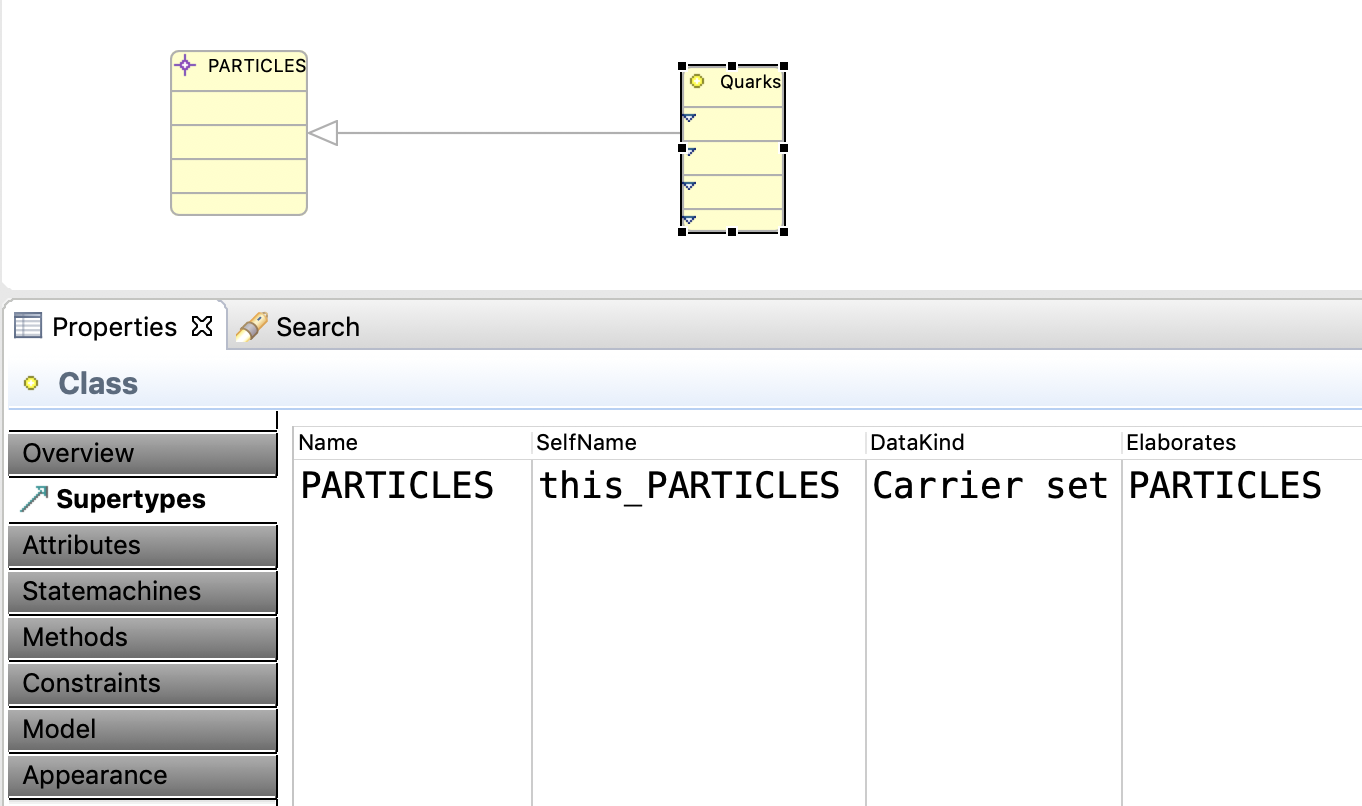
\includegraphics[width=700]{figures/ClassSupertypeSimple.png}
	\else
	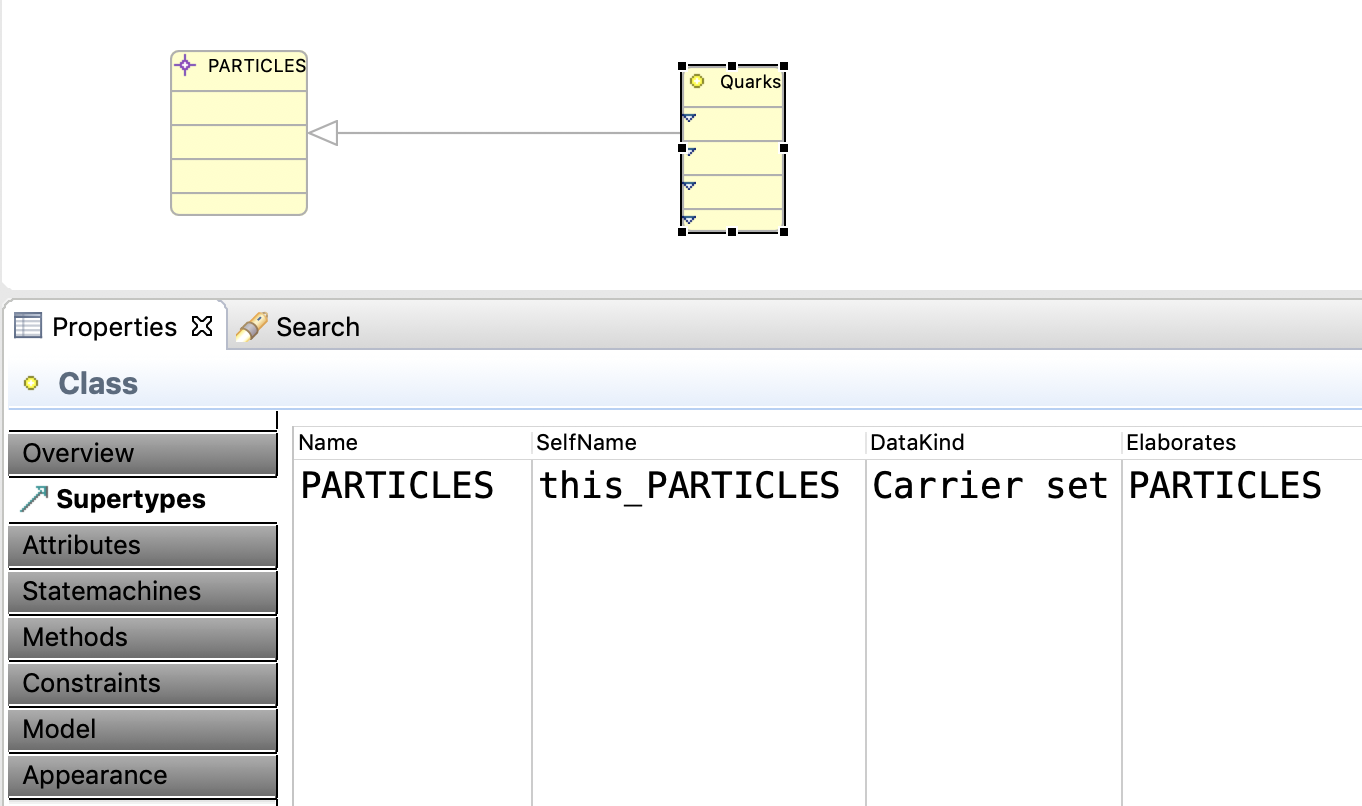
\includegraphics[width=0.7\textwidth]{figures/ClassSupertypeSimple.png}
	\fi
	\caption{Supertype relationship between two classes}
	\label{fig:ClassSupertypeSimple}
\end{figure}

 
\emph{Note: It is more natural to draw supertype relationships on the class diagram, but in Event-B we tend to reverse this relationship and think about subtype relations.
	This is reflected in the translation and also to some extent in the descriptions that follow.}

When several classes have the same supertype the default assumption is that there are no additional constraints to the individual subset relationships. That is, there may be elements of the supertype that are in both subtypes and others that are not in any subtype.
A subtype grouping element is available to specify that a group of subtypes are disjoint, cover all instances or both (partition).
\emph{Note: There is no pallette tool for creating subtype groups; they have to be created using the popup menu for a class. (Use the leftmost icon in the popup shown in Fig.~\ref{fig:CDpopups}).}
Fig.~\ref{fig:ClassSubtypeGroup} shows a group of subtypes and the properties of the group. The default setting is \code{Disjoint} and \code{Cover} (i.e. a partition). The generated Event-B is shown below. 

\begin{figure}[!htbp]
	\centering
	\ifplastex
	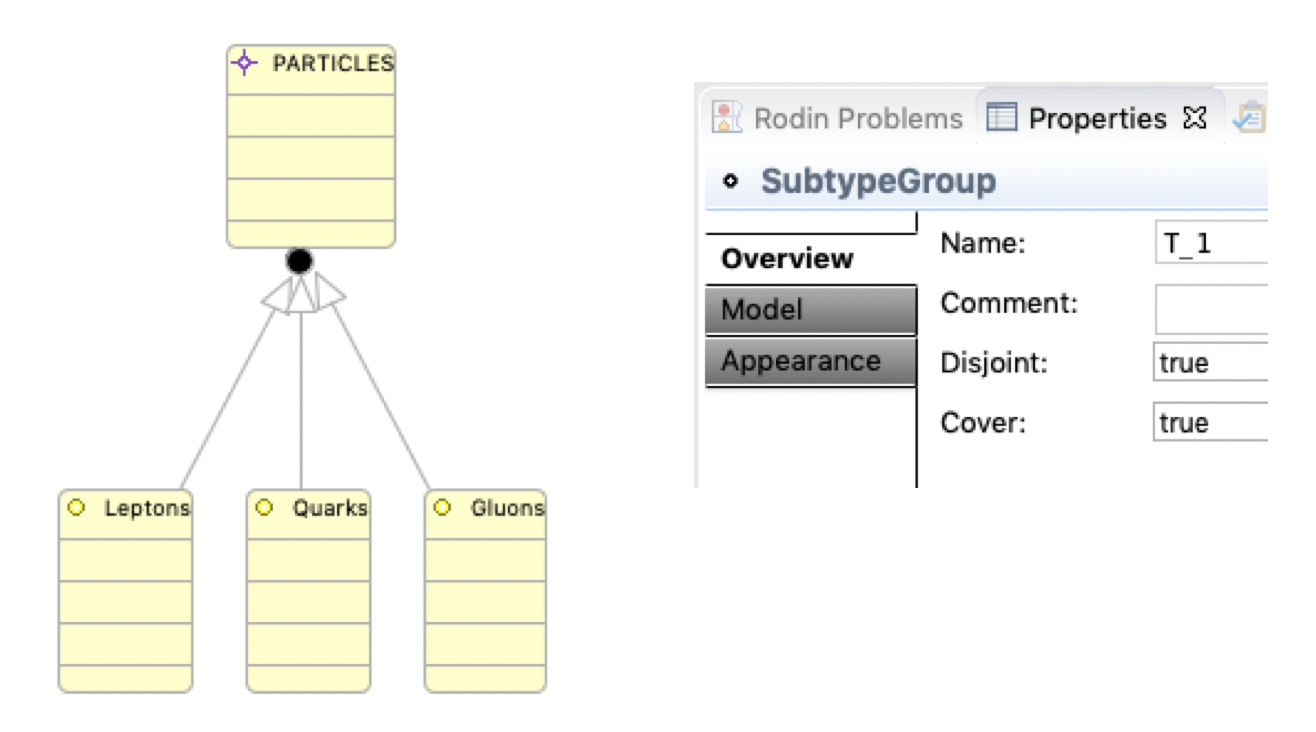
\includegraphics[width=700]{figures/ClassSubtypeGroupPartition.png}
	\else
	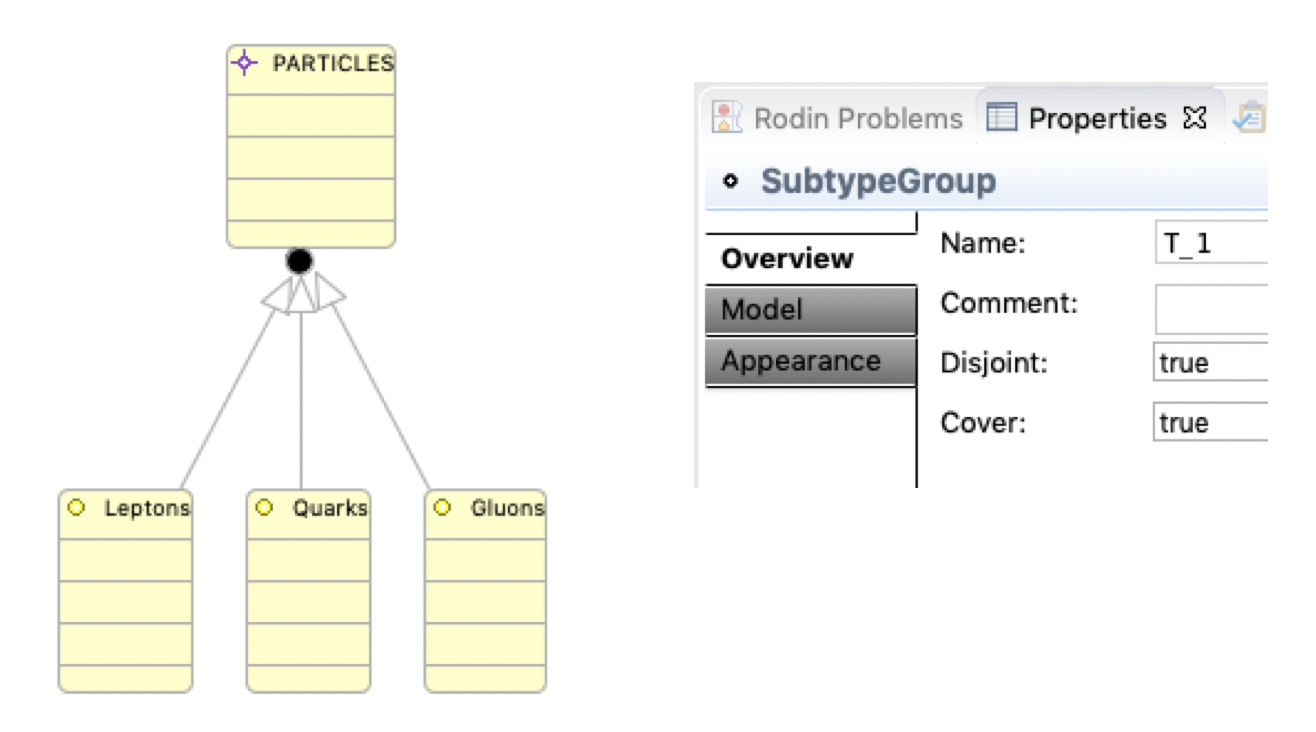
\includegraphics[width=0.7\textwidth]{figures/ClassSubtypeGroupPartition.png}
	\fi
	\caption{Subtype group and its properties}
	\label{fig:ClassSubtypeGroup}
\end{figure}

\CONTEXT{SubtypeGroups}{}{}
\SETS{
	\Set{PARTICLES}{}
}
\CONSTANTS{
	\Constant{Leptons}{}
	\Constant{Quarks}{}
	\Constant{Gluons}{}
}
\AXIOMS{
	\Axiom{subtypeGroup\_T\_1}{false}{$partition(PARTICLES, Leptons, Quarks, Gluons)$}{}
	\Axiom{PARTICLES\_supertypeOf\_Leptons}{false}{$Leptons \in{} \pow{}(PARTICLES)$}{}
	\Axiom{PARTICLES\_supertypeOf\_Quarks}{false}{$Quarks \in{} \pow{}(PARTICLES)$}{}
	\Axiom{PARTICLES\_supertypeOf\_Gluons}{false}{$Gluons \in{} \pow{}(PARTICLES)$}{}
}
\END

When \code{Disjoint = true} and \code{Cover = false}, specifying that the subtypes are disjoint but not a partition, the partition axiom is adjusted to allow for some elements that are in the remainder.
It is also possible to specify \code{Disjoint = false} and \code{Cover = true} giving a predicate over the union of the subtypes.
However, this case is not usually useful.
%\CONTEXT{SubtypeGroups}{}{}
%\AXIOMS{
%		\Axiom{subtypeGroup\_T\_1}{false}{$partition(PARTICLES, Leptons, Quarks, Gluons, PARTICLES\setminus{}(Leptons\bunion{}Quarks\bunion{}Gluons))$}{}
%}
%\END